\documentclass[14pt]{beamer}
%\usepackage[brazil]{babel}
\usepackage[T1]{fontenc}
\usepackage[latin1]{inputenc}
\usepackage{amsmath,amsfonts,amsthm}
\usepackage{amssymb}
\usepackage{stmaryrd}
\usepackage{latexsym}
\usepackage{hyperref}
\usepackage{graphicx}
\usepackage{xcolor}
\usepackage{proof}

\makeatletter
\def\mathcolor#1#{\@mathcolor{#1}}
\def\@mathcolor#1#2#3{%
  \protect\leavevmode
  \begingroup
    \color#1{#2}#3%
  \endgroup
}

\makeatother
\newcommand*{\Scale}[2][4]{\scalebox{#1}{$#2$}}%
\newcommand*{\Resize}[2]{\resizebox{#1}{!}{$#2$}}%
\newcommand{\sembrack}[1]{\ensuremath{\llbracket #1 \rrbracket}}
%\newtheorem{Lemma}{Lemma}
%\newtheorem{Theorem}{Theorem}
\newcommand{\idris}[1]{\texttt{#1}}
\usetheme{Luebeck}

\title{Certified Derivative-based Parsing of Regular Expressions}

\author{Raul Lopes\inst{1} \and Rodrigo Ribeiro \inst{2} \and Carlos Camar\~ao\inst{3}}
\institute{DECOM, Universidade Federal de Ouro Preto (UFOP), Ouro Preto
\and
DECSI, Universidade Federal de Ouro Preto (UFOP), Jo\~ao Monlevade
\and
DCC, Universidade Federal de Minas Gerais (UFMG), Belo Horizonte
}

\date[SBLP 2016]{XX Brazilian Symposium on Programming Languages, 2016}

\begin{document}
     \begin{frame}
         \titlepage
     \end{frame}
     \begin{frame}{Introduction}
        \begin{itemize}
           \item Parsing is a fundamental activity in computing.
           \begin{itemize}
              \item Used by compilers and string search tools
           \end{itemize}
           \item[\ ]
           \item In this work, we focus on parsing Regular Languages (RLs).
           \begin{itemize}
             \item Languages accepted by (non)-deterministic finite automata
             and Regular Expressions (REs).
           \end{itemize}
        \end{itemize}
     \end{frame}
     \begin{frame}{Introduction}
        \begin{itemize}
           \item REs are an algebraic and compact way to specify RLs.
           \item RLs are used in lexical analyser generators and search tools.
           \item Our objective: Formalize an algorithm for RE based search
                 using Dependently typed language Idris.
        \end{itemize}
     \end{frame}
     \begin{frame}{Introduction}
        \begin{itemize}
           \item Our approach is to certify a search algorithm based on
                 Brzozowski derivatives.
           \item Derivatives are an alternative method to compute a equivalent
                 automaton from a given RE.
           \item Some recent works uses derivatives for parsing of both RE and
                 even context free ones.
        \end{itemize}
     \end{frame}
     \begin{frame}{Contributions}
        \begin{itemize}
           \item A complete formalization of derivative based parsing in Idris.
                 The algorithm produces a parse tree that is an evidence that
                 the input string is indeed on RE language or a proof that no
                 such tree exists.
           \item A detailed formalization of the so-called ``smart-constructors''
                used to quotient REs with respect to ACUI-axioms.
        \end{itemize}
     \end{frame}
     \begin{frame}[fragile=singleslide]
        \frametitle{An Overview of Idris}
            \begin{itemize}
               \item Idris is a dependently typed programming language which focus
                     on programming rather than proving.
               \item Idris syntax is similar to Haskell syntax.
               \item Example: Natural numbers in Peano notation.
            \end{itemize}
            \begin{verbatim}
data Nat = Z | S Nat
            \end{verbatim}
     \end{frame}
     \begin{frame}[fragile=singleslide]
        \frametitle{An Overview of Idris}
            \begin{itemize}
               \item Idris supports indexed type families using a Haskell GADT
                     style syntax (similar to Agda's syntax).
               \item Example: Length-indexed lists (aka vectors) and safe head
                     function.
            \end{itemize}
            \begin{verbatim}
data Vec : Nat -> Type -> Type where
    Nil : Vec Z a
    (::) : a -> Vec n a -> Vec (S n) a

head : Vec (S n) a -> a
head (x :: _) = x
            \end{verbatim}
     \end{frame}
     \begin{frame}[fragile=singleslide]
        \frametitle{Regular Expressions}
        \begin{itemize}
           \item REs are defined with respect to a given alphabet, $\Sigma$, by
           the following context-free grammar:
           \[
           e ::= \emptyset\,\mid\,\epsilon\,\mid\,a\,\mid\,e\,e\,\mid\,e+e\,\mid\,e^{\star}
           \]
        \end{itemize}
     \end{frame}
     \begin{frame}[fragile=singleslide]
        \frametitle{Regular Expressions}
           \begin{itemize}
           \item Idris representation
           \begin{verbatim}
data RegExp : Type where
   Zero : RegExp
   Eps  : RegExp
   Chr  : Nat -> RegExp
   Cat  : RegExp -> RegExp -> RegExp
   Alt  : RegExp -> RegExp -> RegExp
   Star : RegExp -> RegExp
           \end{verbatim}
        \end{itemize}
     \end{frame}
     \begin{frame}{Regular Expression Semantics}
        \begin{itemize}
           \item REs semantics as syntax directed judgement:
           \[
              \begin{array}{cc}
                 \infer[]{\epsilon \in \sembrack{\epsilon}}{} &
                 \infer[]{a \in \sembrack{a}}{a \in \Sigma} \\ \\
                 \infer[]{ww' \in \sembrack{ee'}}
                         {w \in \sembrack{e} & w' \in \sembrack{e'}} &
                 \infer[]{w \in \sembrack{e + e'}}{w\in\sembrack{e}}\\ \\
                 \infer[]{w \in \sembrack{e + e'}}{w\in\sembrack{e'}} &
                 \infer[]{w\in \sembrack{e^{\star}}}
                         {w\in\sembrack{\epsilon + ee^{\star}}}
              \end{array}
           \]
        \end{itemize}
     \end{frame}
     \begin{frame}[fragile=singleslide]
        \frametitle{Regular Expression Semantics}
        \begin{verbatim}
data InRegExp : Word -> RegExp -> Type where
   InEps : InRegExp [] Eps
   InChr : InRegExp [ a ] (Chr a)
   InCat : InRegExp xs l ->
           InRegExp ys r ->
           zs = xs ++ ys ->
           InRegExp zs (Cat l r)
   InAltL : InRegExp xs l ->
            InRegExp xs (Alt l r)
   -- some rules omitted...
        \end{verbatim}
     \end{frame}
     \begin{frame}{Nullability Test}
        \begin{itemize}
           \item Brzozowski definition uses an auxiliar function, $\nu(e)$,
                 which returns $\epsilon$ if $\epsilon\in\sembrack{e}$ or
                 $\emptyset$, otherwise.
                 \[
                     \begin{array}{lcl}
                          \nu(\emptyset) & = & \emptyset \\
                          \nu(\epsilon)    & = & \epsilon \\
                          \nu(a)                & = & \emptyset \\
                          \nu(e\,e')           & = & \left\{
                                                                  \begin{array}{ll}
                                                                       \epsilon &
                                                                                  \text{if
                                                                                  }\nu(e)
                                                                                  =
                                                                                  \nu(e')
                                                                                  =
                                                                                  \epsilon
                                                                    \\
                                                                    \emptyset &
                                                                                \text{otherwise}
                                                                  \end{array}
                                                              \right. \\
                          \nu(e + e')  & = & \left\{
                                                          \begin{array}{ll}
                                                               \epsilon & \text{if
                                                                          }\nu(e) =
                                                                          \epsilon
                                                                          \text{ or
                                                                          }\nu(e') =
                                                                          \epsilon \\
                                                               \emptyset & \text{otherwise}
                                                          \end{array}
                                                       \right. \\
                          \nu(e^\star) & = & \epsilon
                     \end{array}
                 \]
        \end{itemize}
     \end{frame}
     \begin{frame}
        \frametitle{Nullability Test}
        \begin{itemize}
           \item Idris implementation of nullability tests shows its decidability.
           \item Theorem \texttt{hasEmptyDec} either returns a proof that
           \texttt{InRegExp Eps e} or an evidence that such construction is
           impossible.
           \begin{itemize}
             \item Theorem follows by induction over RE structure.
           \end{itemize}
        \end{itemize}
     \end{frame}
     \begin{frame}{Smart Constructors}
        \begin{itemize}
           \item Smart constructors ensures the following RE equivalences
           \[
           \begin{array}{lcl}
              1)\: e + \emptyset \approx e &\hspace{1cm} & 2)\: \emptyset + e \approx e\\
              3)\: e\:\emptyset \approx \emptyset & \hspace{1cm} & 4)\: e\:\epsilon \approx e\\
              5)\: \emptyset\:e\approx \emptyset & & 6)\: \epsilon\: e \approx e\\
              7)\: \emptyset^\star \approx \epsilon & \hspace{1cm} & 8)\: \epsilon^\star
                                                 \approx \epsilon \\
          \end{array} \]
        \end{itemize}
     \end{frame}
     \begin{frame}[fragile=singleslide]
        \frametitle{Smart Constructors}
        \begin{itemize}
           \item Smart constructor for union.
           \begin{itemize}
             \item Such smart constructor is sound and complete w.r.t.
                   RE semantics.
             \item Same structure for smart constructors for concatenation and
                   star.
           \end{itemize}
        \end{itemize}
        \begin{verbatim}
(.|.) : RegExp -> RegExp -> RegExp
Zero .|. e = e
e .|. Zero = e
e .|. e'   = Alt e e'
        \end{verbatim}
     \end{frame}
     \begin{frame}{Derivative of Regular Expression}
        \begin{itemize}
           \item Idris version uses nullability test function and smart constructors
                 for concatenation, union and star.
        \end{itemize}
        \[
        \begin{array}{lclr}
          \partial_a(\emptyset) & = & \emptyset\\
          \partial_a(\epsilon) & = & \emptyset \\
          \partial_a(b) & = & \left\{
                              \begin{array}{lr}
                                \epsilon & \text{if } b = a\\
                                \emptyset & \text{otherwise}
                              \end{array}
                                        \right. \\
          \partial_a(e\:e') & = & \partial_a(e)\,e' + \nu(e)\,\partial_a(e')\\
          \partial_a(e + e') & = & \partial_a(e) + \partial_a(e') \\
          \partial_a(e^\star) & = & \partial_a(e)\,e^\star\\
        \end{array}
        \]
     \end{frame}
     \begin{frame}{Derivative Properties}
        \begin{Theorem}[Soundness of derivative operation]\label{derivsound}
        For all RE \idris{e}, string \idris{xs} and symbol \idris{x}, if
        \idris{InRegExp xs (deriv x e)} then \idris{InRegExp (x :: xs) e}.
        \end{Theorem}
        \begin{proof}
          By induction on the structure of \idris{e}, using the soundness
          lemmas for smart constructors and decidability of the emptiness
          test.
        \end{proof}
     \end{frame}
     \begin{frame}{Derivative Properties}
        \begin{Theorem}[Completeness of derivative operation]\label{derivcomplete}
        For all RE \idris{e}, string \idris{xs} and symbol \idris{x}, if
        \idris{InRegExp (x :: xs) e} then \idris{InRegExp xs (deriv e x)}.
        \end{Theorem}
        \begin{proof}
          By induction on the structure of \idris{e} using the completeness
          lemmas for smart constructors and decidability of the emptiness
          test.
        \end{proof}
     \end{frame}
     \begin{frame}{Parsing with Derivatives}
        \begin{itemize}
           \item Just apply the derivative operation recursively on each symbol
           of input.
           \item String accepted if resulting RE is nullable. Our implementation
           keeps track if a prefix or a substring of input is matched by input RE.
        \end{itemize}
        \[
        \begin{array}{lcl}
          \partial_\epsilon^\star(e) & = & e\\
          \partial_{a\,w}^\star(e) & = & \partial_w^\star(\partial_a(e))\\
        \end{array}
        \]
     \end{frame}
     \begin{frame}{Experiments}
        \begin{figure}[!ht]
            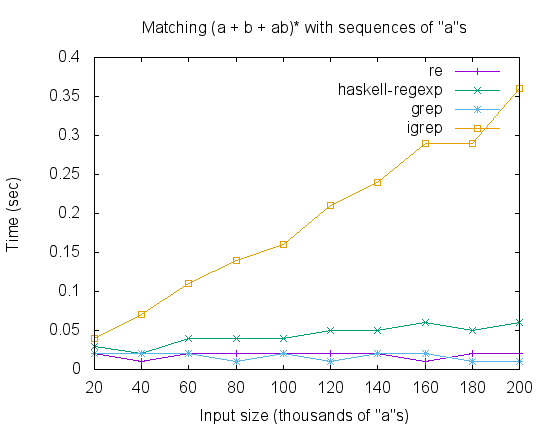
\includegraphics[width=0.9\textwidth]{as.png}
           \centering
           %\caption{Results of experiment 1.}
           \label{fig:graph1}
        \end{figure}
     \end{frame}
     \begin{frame}{Experiments}
        \begin{figure}[!ht]
           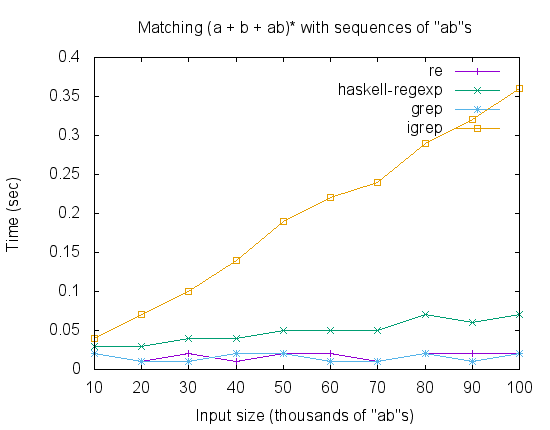
\includegraphics[width=0.9\textwidth]{abs.png}
         \centering
         %\caption{Results of experiment 2.}
         \label{fig:graph2}
        \end{figure}
     \end{frame}
     \begin{frame}{Conclusion and Future Work}
        \begin{itemize}
           \item Complete formalization of derivative based RE parsing algorithm in Idris.
           \item A tool, named iGrep, is produced from the formalization and experiments were
           conducted.
           \item Future work:
           \begin{itemize}
             \item Improve efficient by using disambiguation strategies like
            greedy or POSIX.
             \item Compile RE to an automaton and use it to parse input string and compare
                the efficency with derivative based algorithm.
             \end{itemize}
        \end{itemize}
     \end{frame}
\end{document}
